

\def\qtr{Summer 2019}
\def\due{Monday, July 15 at 11:59 pm}
\def\piazza{\url{http://piazza.com/stanford/summer2019/cs229}}
\def\psetnum{1 }

%%% Change the following flag to toggle between questions or solutions

%\def\solutions{1}


\documentclass{article}

\usepackage{graphicx}

\newcommand{\di}{{d}}
\newcommand{\nexp}{{n}}
\newcommand{\nf}{{p}}
\newcommand{\vcd}{{\textbf{D}}}

\usepackage{graphicx,caption}
\usepackage{enumitem}
\usepackage{epstopdf,subcaption}
\usepackage{psfrag}
\usepackage{amsmath,amssymb,epsf}
\usepackage{verbatim}
\usepackage[hyphens]{url}
\usepackage{color}
\usepackage{bbm}
\usepackage{listings}
\usepackage{setspace}
\usepackage{float}
\definecolor{Code}{rgb}{0,0,0}
\definecolor{Decorators}{rgb}{0.5,0.5,0.5}
\definecolor{Numbers}{rgb}{0.5,0,0}
\definecolor{MatchingBrackets}{rgb}{0.25,0.5,0.5}
\definecolor{Keywords}{rgb}{0,0,1}
\definecolor{self}{rgb}{0,0,0}
\definecolor{Strings}{rgb}{0,0.63,0}
\definecolor{Comments}{rgb}{0,0.63,1}
\definecolor{Backquotes}{rgb}{0,0,0}
\definecolor{Classname}{rgb}{0,0,0}
\definecolor{FunctionName}{rgb}{0,0,0}
\definecolor{Operators}{rgb}{0,0,0}
\definecolor{Background}{rgb}{0.98,0.98,0.98}
\lstdefinelanguage{Python}{
numbers=left,
numberstyle=\footnotesize,
numbersep=1em,
xleftmargin=1em,
framextopmargin=2em,
framexbottommargin=2em,
showspaces=false,
showtabs=false,
showstringspaces=false,
frame=l,
tabsize=4,
% Basic
basicstyle=\ttfamily\footnotesize\setstretch{1},
backgroundcolor=\color{Background},
% Comments
commentstyle=\color{Comments}\slshape,
% Strings
stringstyle=\color{Strings},
morecomment=[s][\color{Strings}]{"""}{"""},
morecomment=[s][\color{Strings}]{'''}{'''},
% keywords
morekeywords={import,from,class,def,for,while,if,is,in,elif,else,not,and,or
,print,break,continue,return,True,False,None,access,as,,del,except,exec
,finally,global,import,lambda,pass,print,raise,try,assert},
keywordstyle={\color{Keywords}\bfseries},
% additional keywords
morekeywords={[2]@invariant},
keywordstyle={[2]\color{Decorators}\slshape},
emph={self},
emphstyle={\color{self}\slshape},
%
}


\pagestyle{empty} \addtolength{\textwidth}{1.0in}
\addtolength{\textheight}{0.5in}
\addtolength{\oddsidemargin}{-0.5in}
\addtolength{\evensidemargin}{-0.5in}
\newcommand{\ruleskip}{\bigskip\hrule\bigskip}
\newcommand{\nodify}[1]{{\sc #1}}
\newcommand{\points}[1]{{\textbf{[#1 points]}}}
\newcommand{\subquestionpoints}[1]{{[#1 points]}}
\newenvironment{answer}{{\bf Answer:} \sf \begingroup\color{red}}{\endgroup}%

\newcommand{\bitem}{\begin{list}{$\bullet$}%
{\setlength{\itemsep}{0pt}\setlength{\topsep}{0pt}%
\setlength{\rightmargin}{0pt}}}
\newcommand{\eitem}{\end{list}}

\setlength{\parindent}{0pt} \setlength{\parskip}{0.5ex}
\setlength{\unitlength}{1cm}

\renewcommand{\Re}{{\mathbb R}}
\newcommand{\R}{\mathbb{R}}
\newcommand{\what}[1]{\widehat{#1}}

\renewcommand{\comment}[1]{}
\newcommand{\mc}[1]{\mathcal{#1}}
\newcommand{\half}{\frac{1}{2}}

\def\KL{D_{KL}}
\def\xsi{x^{(i)}}
\def\ysi{y^{(i)}}
\def\zsi{z^{(i)}}
\def\E{\mathbb{E}}

\usepackage{tikz}
\usepackage{bbding}
\usepackage{pifont}
\usepackage{wasysym}
\usepackage{amssymb}




\begin{document}

\pagestyle{myheadings} \markboth{}{CS229 Problem Set \#\psetnum}

\ifnum\solutions=1{
{\huge\noindent CS 229, \qtr\\
Problem Set \#\psetnum Solutions}\\\\
Makanov Artem Zhanovich(\texttt{YOUR SUNET HERE})
} \else {\huge
\noindent CS 229, \qtr\\
Problem Set \#\psetnum
} \fi

\ruleskip

{\bf Due {\due } on Gradescope.}

\medskip

\item \points{20} {\bf K-means for compression}

In this problem, we will apply the K-means algorithm to lossy image
compression, by reducing the number of colors used in an image.

We will be using the files \texttt{src/k\_means/peppers-small.tiff} and \texttt{src/k\_means/peppers-large.tiff}.
	

The \texttt{peppers-large.tiff} file contains
a 512x512 image of peppers represented in 24-bit color. This means
that, for each of the 262144 pixels in the image, there are three
8-bit numbers (each ranging from 0 to 255) that represent the red,
green, and blue intensity values for that pixel. The straightforward
representation of this image therefore takes about $262144 \times 3 =
786432$ bytes (a byte being 8 bits). To compress the image, we will
use K-means to reduce the image to $k = 16$ colors. More specifically,
each pixel in the image is considered a point in the three-dimensional
$(r, g, b)$-space. To compress the image, we will cluster these points
in color-space into 16 clusters, and replace each pixel with the
closest cluster centroid.

Follow the instructions below. Be warned that some of these operations
can take a while (several minutes even on a fast computer)!


\begin{enumerate}

  \item\subquestionpoints{15}
\textbf{[Coding Problem] K-Means Compression Implementation.}
First let us \emph{look} at our data. From the \texttt{src/k\_means/} directory, open an interactive Python prompt, and type
%
\begin{center}
  \texttt{from matplotlib.image import imread; import matplotlib.pyplot as plt;}
\end{center}
%
and run \texttt{A = imread(`peppers-large.tiff')}. Now, \texttt{A} is a ``three dimensional matrix,'' and \texttt{A[:,:,0]}, \texttt{A[:,:,1]} and \texttt{A[:,:,2]} are 512x512 arrays that respectively contain the red, green, and blue values for each pixel. Enter \texttt{plt.imshow(A); plt.show()} to display the image.

Since the large image has 262,144 pixels and would take a while to cluster, we will instead run vector quantization on a smaller image. Repeat (a) with \texttt{peppers-small.tiff}.


Next we will implement image compression in the file \texttt{src/k\_means/k\_means.py} which has some starter code. Treating each pixel's $(r, g, b)$ values as an element of $\Re^3$, implement K-means with 16 clusters on the pixel data from this smaller image, iterating (preferably) to convergence, but in no case for less than 30 iterations. For initialization, set each cluster centroid to the $(r, g, b)$-values of a randomly chosen pixel in the image.

Take the image of \texttt{peppers-large.tiff}, and replace each pixel's $(r, g, b)$ values with the value of the closest cluster centroid from the set of centroids computed with \texttt{peppers-small.tiff}. Visually compare it to the original image to verify that your implementation is reasonable. \textbf{Include in your write-up a copy of this compressed image alongside the original image.}


\ifnum\solutions=1 {
  \begin{answer}
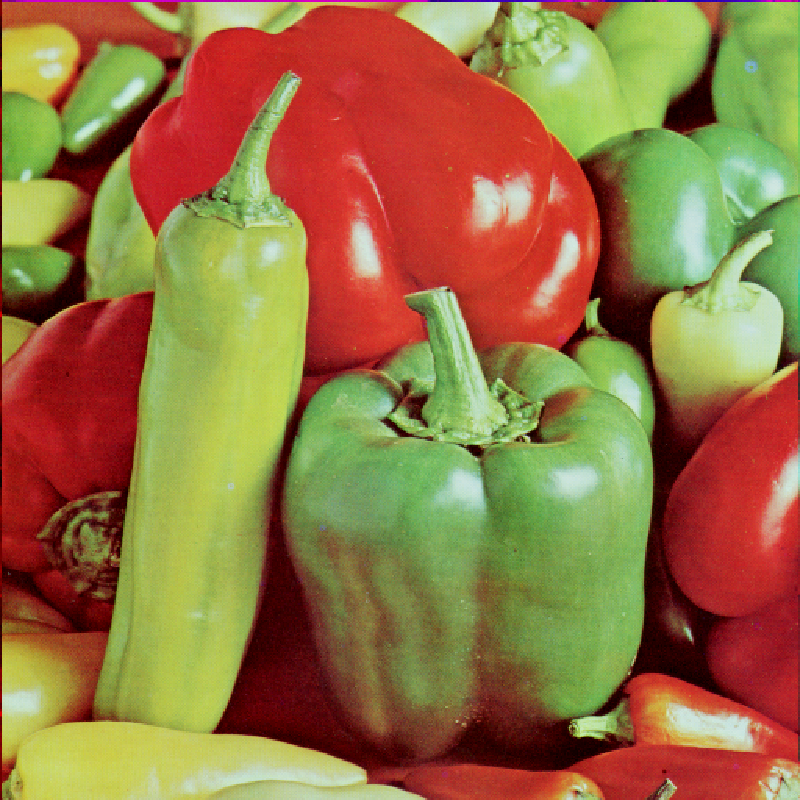
\includegraphics[width=0.5\textwidth]{peppers-large.pdf}
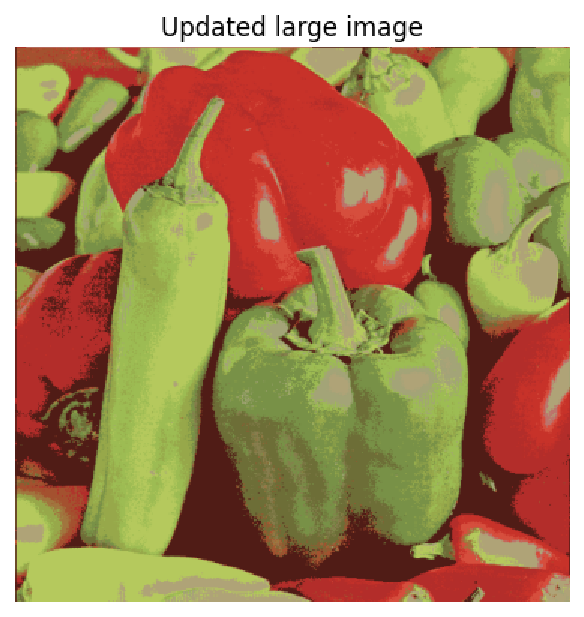
\includegraphics[width=0.5\textwidth]{updated_large.pdf}
\end{answer}

} \fi


  \item\subquestionpoints{5} \textbf{Compression Factor.}

If we represent the image with these reduced (16) colors, by
(approximately) what factor have we compressed the image?


\ifnum\solutions=1 {
  \begin{answer}
The original picture requieres 3*8=24 bits to represent one pixel. New compressed picture requires 4 bits. 24/4=6.
\end{answer}

} \fi

\end{enumerate}



\begin{enumerate}[wide, labelwidth=!, labelindent=0pt]

\clearpage
\item \points{20} {\bf K-means for compression}

In this problem, we will apply the K-means algorithm to lossy image
compression, by reducing the number of colors used in an image.

We will be using the files \texttt{src/k\_means/peppers-small.tiff} and \texttt{src/k\_means/peppers-large.tiff}.
	

The \texttt{peppers-large.tiff} file contains
a 512x512 image of peppers represented in 24-bit color. This means
that, for each of the 262144 pixels in the image, there are three
8-bit numbers (each ranging from 0 to 255) that represent the red,
green, and blue intensity values for that pixel. The straightforward
representation of this image therefore takes about $262144 \times 3 =
786432$ bytes (a byte being 8 bits). To compress the image, we will
use K-means to reduce the image to $k = 16$ colors. More specifically,
each pixel in the image is considered a point in the three-dimensional
$(r, g, b)$-space. To compress the image, we will cluster these points
in color-space into 16 clusters, and replace each pixel with the
closest cluster centroid.

Follow the instructions below. Be warned that some of these operations
can take a while (several minutes even on a fast computer)!


\begin{enumerate}

  \item\subquestionpoints{15}
\textbf{[Coding Problem] K-Means Compression Implementation.}
First let us \emph{look} at our data. From the \texttt{src/k\_means/} directory, open an interactive Python prompt, and type
%
\begin{center}
  \texttt{from matplotlib.image import imread; import matplotlib.pyplot as plt;}
\end{center}
%
and run \texttt{A = imread(`peppers-large.tiff')}. Now, \texttt{A} is a ``three dimensional matrix,'' and \texttt{A[:,:,0]}, \texttt{A[:,:,1]} and \texttt{A[:,:,2]} are 512x512 arrays that respectively contain the red, green, and blue values for each pixel. Enter \texttt{plt.imshow(A); plt.show()} to display the image.

Since the large image has 262,144 pixels and would take a while to cluster, we will instead run vector quantization on a smaller image. Repeat (a) with \texttt{peppers-small.tiff}.


Next we will implement image compression in the file \texttt{src/k\_means/k\_means.py} which has some starter code. Treating each pixel's $(r, g, b)$ values as an element of $\Re^3$, implement K-means with 16 clusters on the pixel data from this smaller image, iterating (preferably) to convergence, but in no case for less than 30 iterations. For initialization, set each cluster centroid to the $(r, g, b)$-values of a randomly chosen pixel in the image.

Take the image of \texttt{peppers-large.tiff}, and replace each pixel's $(r, g, b)$ values with the value of the closest cluster centroid from the set of centroids computed with \texttt{peppers-small.tiff}. Visually compare it to the original image to verify that your implementation is reasonable. \textbf{Include in your write-up a copy of this compressed image alongside the original image.}


\ifnum\solutions=1 {
  \begin{answer}
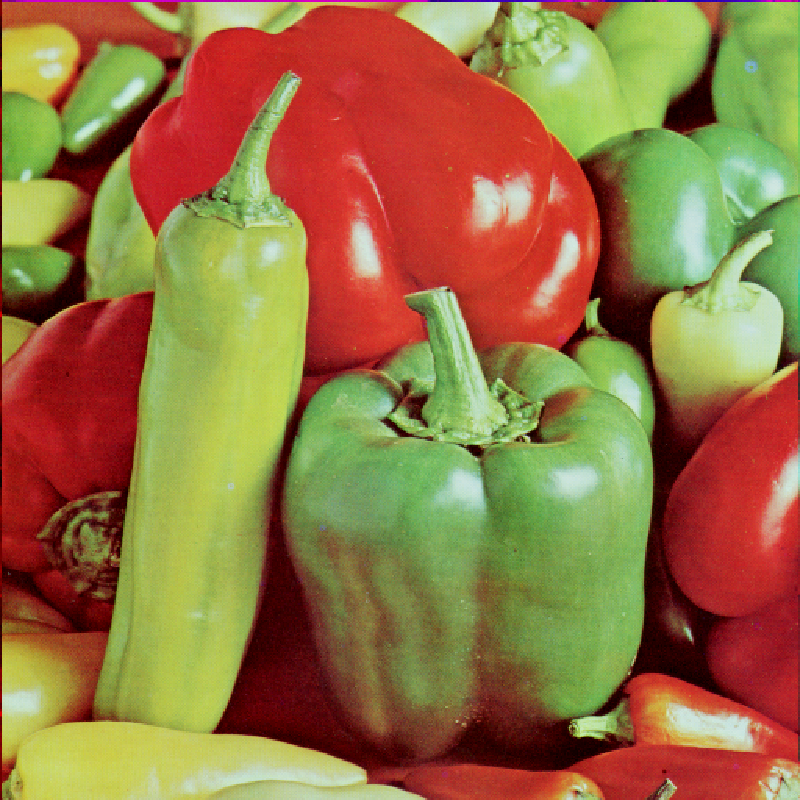
\includegraphics[width=0.5\textwidth]{peppers-large.pdf}
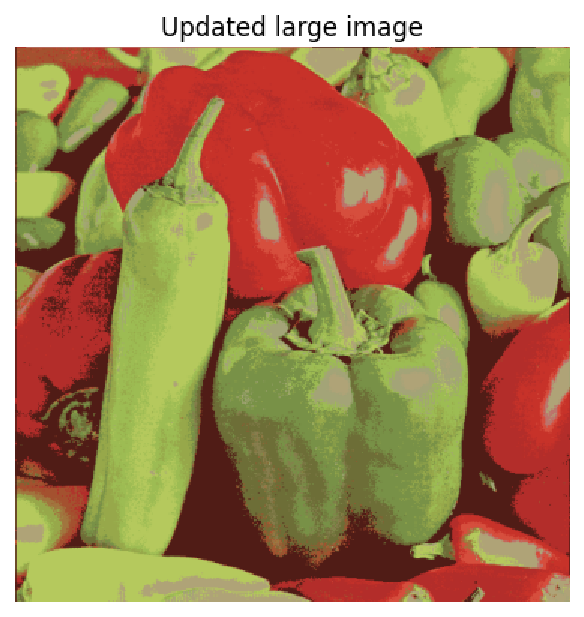
\includegraphics[width=0.5\textwidth]{updated_large.pdf}
\end{answer}

} \fi


  \item\subquestionpoints{5} \textbf{Compression Factor.}

If we represent the image with these reduced (16) colors, by
(approximately) what factor have we compressed the image?


\ifnum\solutions=1 {
  \begin{answer}
The original picture requieres 3*8=24 bits to represent one pixel. New compressed picture requires 4 bits. 24/4=6.
\end{answer}

} \fi

\end{enumerate}



\clearpage
\item \points{20} {\bf K-means for compression}

In this problem, we will apply the K-means algorithm to lossy image
compression, by reducing the number of colors used in an image.

We will be using the files \texttt{src/k\_means/peppers-small.tiff} and \texttt{src/k\_means/peppers-large.tiff}.
	

The \texttt{peppers-large.tiff} file contains
a 512x512 image of peppers represented in 24-bit color. This means
that, for each of the 262144 pixels in the image, there are three
8-bit numbers (each ranging from 0 to 255) that represent the red,
green, and blue intensity values for that pixel. The straightforward
representation of this image therefore takes about $262144 \times 3 =
786432$ bytes (a byte being 8 bits). To compress the image, we will
use K-means to reduce the image to $k = 16$ colors. More specifically,
each pixel in the image is considered a point in the three-dimensional
$(r, g, b)$-space. To compress the image, we will cluster these points
in color-space into 16 clusters, and replace each pixel with the
closest cluster centroid.

Follow the instructions below. Be warned that some of these operations
can take a while (several minutes even on a fast computer)!


\begin{enumerate}

  \item\subquestionpoints{15}
\textbf{[Coding Problem] K-Means Compression Implementation.}
First let us \emph{look} at our data. From the \texttt{src/k\_means/} directory, open an interactive Python prompt, and type
%
\begin{center}
  \texttt{from matplotlib.image import imread; import matplotlib.pyplot as plt;}
\end{center}
%
and run \texttt{A = imread(`peppers-large.tiff')}. Now, \texttt{A} is a ``three dimensional matrix,'' and \texttt{A[:,:,0]}, \texttt{A[:,:,1]} and \texttt{A[:,:,2]} are 512x512 arrays that respectively contain the red, green, and blue values for each pixel. Enter \texttt{plt.imshow(A); plt.show()} to display the image.

Since the large image has 262,144 pixels and would take a while to cluster, we will instead run vector quantization on a smaller image. Repeat (a) with \texttt{peppers-small.tiff}.


Next we will implement image compression in the file \texttt{src/k\_means/k\_means.py} which has some starter code. Treating each pixel's $(r, g, b)$ values as an element of $\Re^3$, implement K-means with 16 clusters on the pixel data from this smaller image, iterating (preferably) to convergence, but in no case for less than 30 iterations. For initialization, set each cluster centroid to the $(r, g, b)$-values of a randomly chosen pixel in the image.

Take the image of \texttt{peppers-large.tiff}, and replace each pixel's $(r, g, b)$ values with the value of the closest cluster centroid from the set of centroids computed with \texttt{peppers-small.tiff}. Visually compare it to the original image to verify that your implementation is reasonable. \textbf{Include in your write-up a copy of this compressed image alongside the original image.}


\ifnum\solutions=1 {
  \begin{answer}
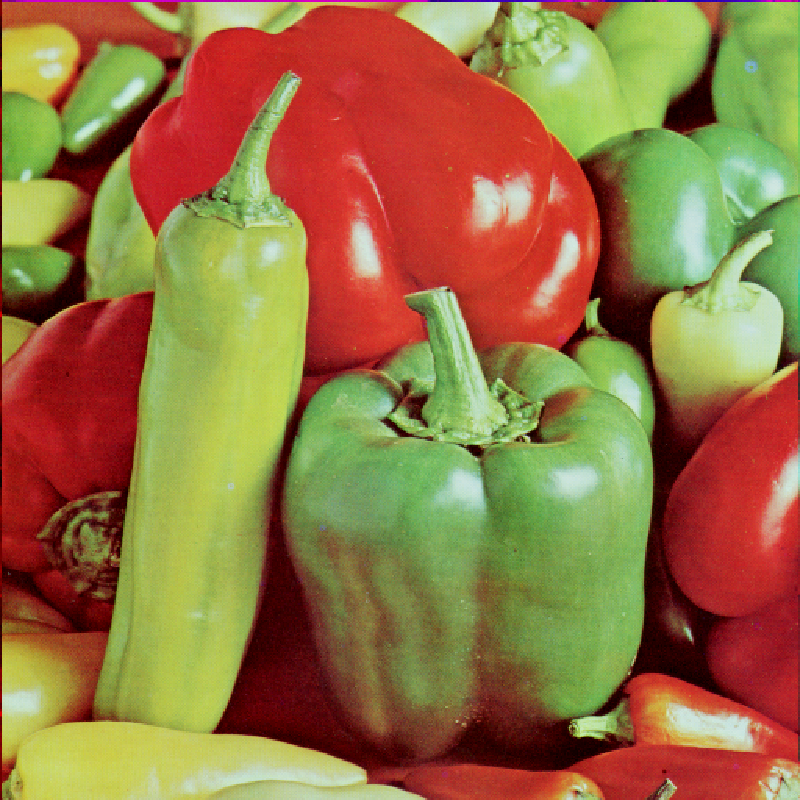
\includegraphics[width=0.5\textwidth]{peppers-large.pdf}
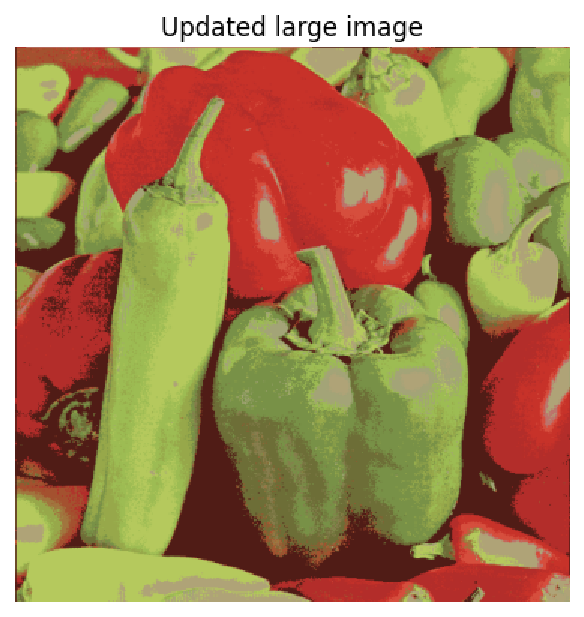
\includegraphics[width=0.5\textwidth]{updated_large.pdf}
\end{answer}

} \fi


  \item\subquestionpoints{5} \textbf{Compression Factor.}

If we represent the image with these reduced (16) colors, by
(approximately) what factor have we compressed the image?


\ifnum\solutions=1 {
  \begin{answer}
The original picture requieres 3*8=24 bits to represent one pixel. New compressed picture requires 4 bits. 24/4=6.
\end{answer}

} \fi

\end{enumerate}



\clearpage
\item \points{20} {\bf K-means for compression}

In this problem, we will apply the K-means algorithm to lossy image
compression, by reducing the number of colors used in an image.

We will be using the files \texttt{src/k\_means/peppers-small.tiff} and \texttt{src/k\_means/peppers-large.tiff}.
	

The \texttt{peppers-large.tiff} file contains
a 512x512 image of peppers represented in 24-bit color. This means
that, for each of the 262144 pixels in the image, there are three
8-bit numbers (each ranging from 0 to 255) that represent the red,
green, and blue intensity values for that pixel. The straightforward
representation of this image therefore takes about $262144 \times 3 =
786432$ bytes (a byte being 8 bits). To compress the image, we will
use K-means to reduce the image to $k = 16$ colors. More specifically,
each pixel in the image is considered a point in the three-dimensional
$(r, g, b)$-space. To compress the image, we will cluster these points
in color-space into 16 clusters, and replace each pixel with the
closest cluster centroid.

Follow the instructions below. Be warned that some of these operations
can take a while (several minutes even on a fast computer)!


\begin{enumerate}

  \item\subquestionpoints{15}
\textbf{[Coding Problem] K-Means Compression Implementation.}
First let us \emph{look} at our data. From the \texttt{src/k\_means/} directory, open an interactive Python prompt, and type
%
\begin{center}
  \texttt{from matplotlib.image import imread; import matplotlib.pyplot as plt;}
\end{center}
%
and run \texttt{A = imread(`peppers-large.tiff')}. Now, \texttt{A} is a ``three dimensional matrix,'' and \texttt{A[:,:,0]}, \texttt{A[:,:,1]} and \texttt{A[:,:,2]} are 512x512 arrays that respectively contain the red, green, and blue values for each pixel. Enter \texttt{plt.imshow(A); plt.show()} to display the image.

Since the large image has 262,144 pixels and would take a while to cluster, we will instead run vector quantization on a smaller image. Repeat (a) with \texttt{peppers-small.tiff}.


Next we will implement image compression in the file \texttt{src/k\_means/k\_means.py} which has some starter code. Treating each pixel's $(r, g, b)$ values as an element of $\Re^3$, implement K-means with 16 clusters on the pixel data from this smaller image, iterating (preferably) to convergence, but in no case for less than 30 iterations. For initialization, set each cluster centroid to the $(r, g, b)$-values of a randomly chosen pixel in the image.

Take the image of \texttt{peppers-large.tiff}, and replace each pixel's $(r, g, b)$ values with the value of the closest cluster centroid from the set of centroids computed with \texttt{peppers-small.tiff}. Visually compare it to the original image to verify that your implementation is reasonable. \textbf{Include in your write-up a copy of this compressed image alongside the original image.}


\ifnum\solutions=1 {
  \begin{answer}
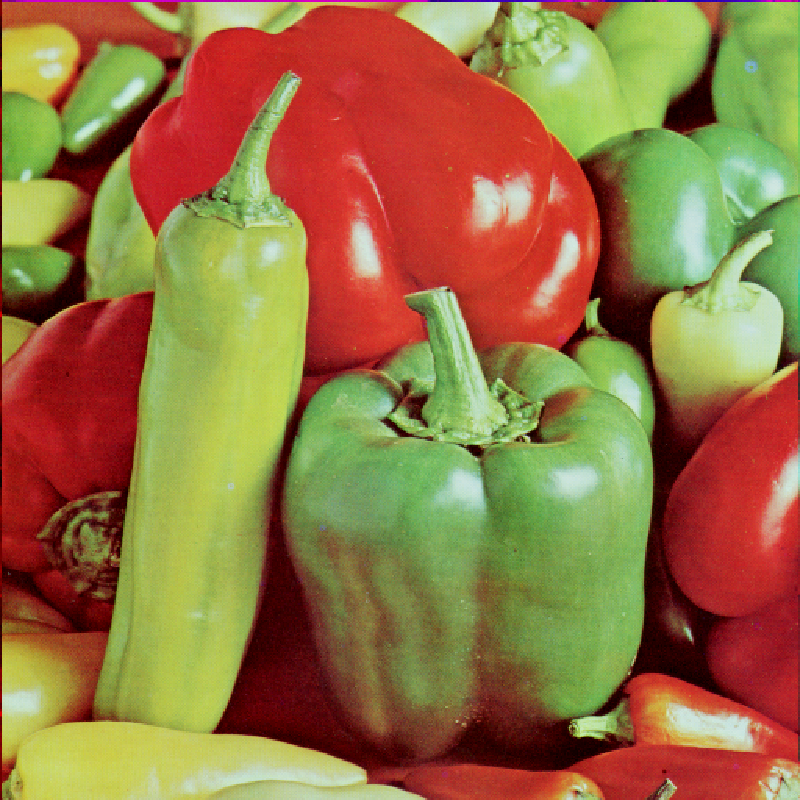
\includegraphics[width=0.5\textwidth]{peppers-large.pdf}
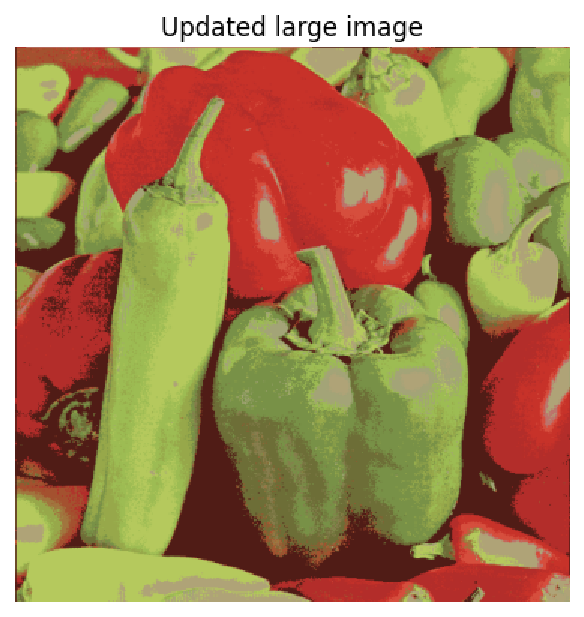
\includegraphics[width=0.5\textwidth]{updated_large.pdf}
\end{answer}

} \fi


  \item\subquestionpoints{5} \textbf{Compression Factor.}

If we represent the image with these reduced (16) colors, by
(approximately) what factor have we compressed the image?


\ifnum\solutions=1 {
  \begin{answer}
The original picture requieres 3*8=24 bits to represent one pixel. New compressed picture requires 4 bits. 24/4=6.
\end{answer}

} \fi

\end{enumerate}



\clearpage
\item \points{20} {\bf K-means for compression}

In this problem, we will apply the K-means algorithm to lossy image
compression, by reducing the number of colors used in an image.

We will be using the files \texttt{src/k\_means/peppers-small.tiff} and \texttt{src/k\_means/peppers-large.tiff}.
	

The \texttt{peppers-large.tiff} file contains
a 512x512 image of peppers represented in 24-bit color. This means
that, for each of the 262144 pixels in the image, there are three
8-bit numbers (each ranging from 0 to 255) that represent the red,
green, and blue intensity values for that pixel. The straightforward
representation of this image therefore takes about $262144 \times 3 =
786432$ bytes (a byte being 8 bits). To compress the image, we will
use K-means to reduce the image to $k = 16$ colors. More specifically,
each pixel in the image is considered a point in the three-dimensional
$(r, g, b)$-space. To compress the image, we will cluster these points
in color-space into 16 clusters, and replace each pixel with the
closest cluster centroid.

Follow the instructions below. Be warned that some of these operations
can take a while (several minutes even on a fast computer)!


\begin{enumerate}

  \item\subquestionpoints{15}
\textbf{[Coding Problem] K-Means Compression Implementation.}
First let us \emph{look} at our data. From the \texttt{src/k\_means/} directory, open an interactive Python prompt, and type
%
\begin{center}
  \texttt{from matplotlib.image import imread; import matplotlib.pyplot as plt;}
\end{center}
%
and run \texttt{A = imread(`peppers-large.tiff')}. Now, \texttt{A} is a ``three dimensional matrix,'' and \texttt{A[:,:,0]}, \texttt{A[:,:,1]} and \texttt{A[:,:,2]} are 512x512 arrays that respectively contain the red, green, and blue values for each pixel. Enter \texttt{plt.imshow(A); plt.show()} to display the image.

Since the large image has 262,144 pixels and would take a while to cluster, we will instead run vector quantization on a smaller image. Repeat (a) with \texttt{peppers-small.tiff}.


Next we will implement image compression in the file \texttt{src/k\_means/k\_means.py} which has some starter code. Treating each pixel's $(r, g, b)$ values as an element of $\Re^3$, implement K-means with 16 clusters on the pixel data from this smaller image, iterating (preferably) to convergence, but in no case for less than 30 iterations. For initialization, set each cluster centroid to the $(r, g, b)$-values of a randomly chosen pixel in the image.

Take the image of \texttt{peppers-large.tiff}, and replace each pixel's $(r, g, b)$ values with the value of the closest cluster centroid from the set of centroids computed with \texttt{peppers-small.tiff}. Visually compare it to the original image to verify that your implementation is reasonable. \textbf{Include in your write-up a copy of this compressed image alongside the original image.}


\ifnum\solutions=1 {
  \begin{answer}
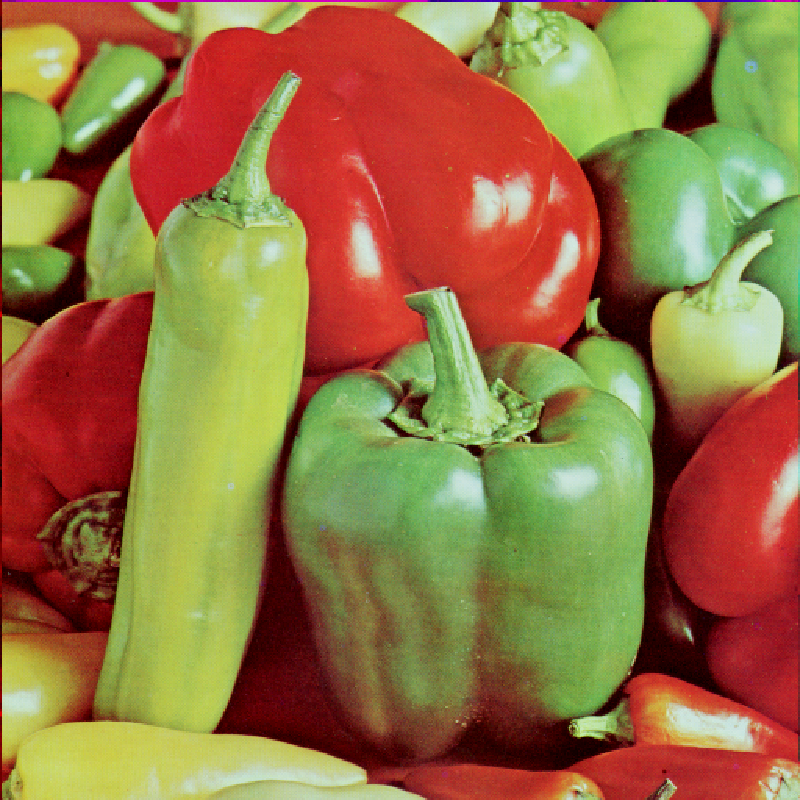
\includegraphics[width=0.5\textwidth]{peppers-large.pdf}
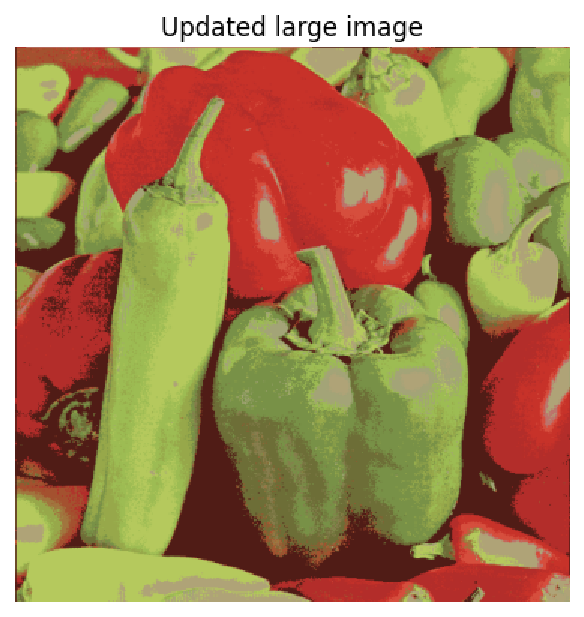
\includegraphics[width=0.5\textwidth]{updated_large.pdf}
\end{answer}

} \fi


  \item\subquestionpoints{5} \textbf{Compression Factor.}

If we represent the image with these reduced (16) colors, by
(approximately) what factor have we compressed the image?


\ifnum\solutions=1 {
  \begin{answer}
The original picture requieres 3*8=24 bits to represent one pixel. New compressed picture requires 4 bits. 24/4=6.
\end{answer}

} \fi

\end{enumerate}



\clearpage
\item \points{20} {\bf K-means for compression}

In this problem, we will apply the K-means algorithm to lossy image
compression, by reducing the number of colors used in an image.

We will be using the files \texttt{src/k\_means/peppers-small.tiff} and \texttt{src/k\_means/peppers-large.tiff}.
	

The \texttt{peppers-large.tiff} file contains
a 512x512 image of peppers represented in 24-bit color. This means
that, for each of the 262144 pixels in the image, there are three
8-bit numbers (each ranging from 0 to 255) that represent the red,
green, and blue intensity values for that pixel. The straightforward
representation of this image therefore takes about $262144 \times 3 =
786432$ bytes (a byte being 8 bits). To compress the image, we will
use K-means to reduce the image to $k = 16$ colors. More specifically,
each pixel in the image is considered a point in the three-dimensional
$(r, g, b)$-space. To compress the image, we will cluster these points
in color-space into 16 clusters, and replace each pixel with the
closest cluster centroid.

Follow the instructions below. Be warned that some of these operations
can take a while (several minutes even on a fast computer)!


\begin{enumerate}

  \item\subquestionpoints{15}
\textbf{[Coding Problem] K-Means Compression Implementation.}
First let us \emph{look} at our data. From the \texttt{src/k\_means/} directory, open an interactive Python prompt, and type
%
\begin{center}
  \texttt{from matplotlib.image import imread; import matplotlib.pyplot as plt;}
\end{center}
%
and run \texttt{A = imread(`peppers-large.tiff')}. Now, \texttt{A} is a ``three dimensional matrix,'' and \texttt{A[:,:,0]}, \texttt{A[:,:,1]} and \texttt{A[:,:,2]} are 512x512 arrays that respectively contain the red, green, and blue values for each pixel. Enter \texttt{plt.imshow(A); plt.show()} to display the image.

Since the large image has 262,144 pixels and would take a while to cluster, we will instead run vector quantization on a smaller image. Repeat (a) with \texttt{peppers-small.tiff}.


Next we will implement image compression in the file \texttt{src/k\_means/k\_means.py} which has some starter code. Treating each pixel's $(r, g, b)$ values as an element of $\Re^3$, implement K-means with 16 clusters on the pixel data from this smaller image, iterating (preferably) to convergence, but in no case for less than 30 iterations. For initialization, set each cluster centroid to the $(r, g, b)$-values of a randomly chosen pixel in the image.

Take the image of \texttt{peppers-large.tiff}, and replace each pixel's $(r, g, b)$ values with the value of the closest cluster centroid from the set of centroids computed with \texttt{peppers-small.tiff}. Visually compare it to the original image to verify that your implementation is reasonable. \textbf{Include in your write-up a copy of this compressed image alongside the original image.}


\ifnum\solutions=1 {
  \begin{answer}
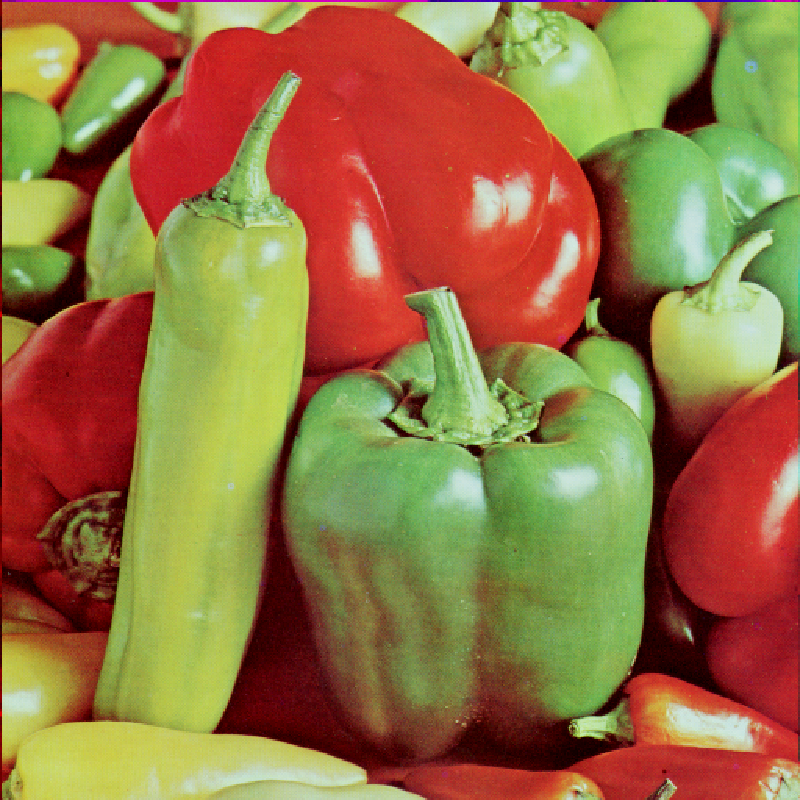
\includegraphics[width=0.5\textwidth]{peppers-large.pdf}
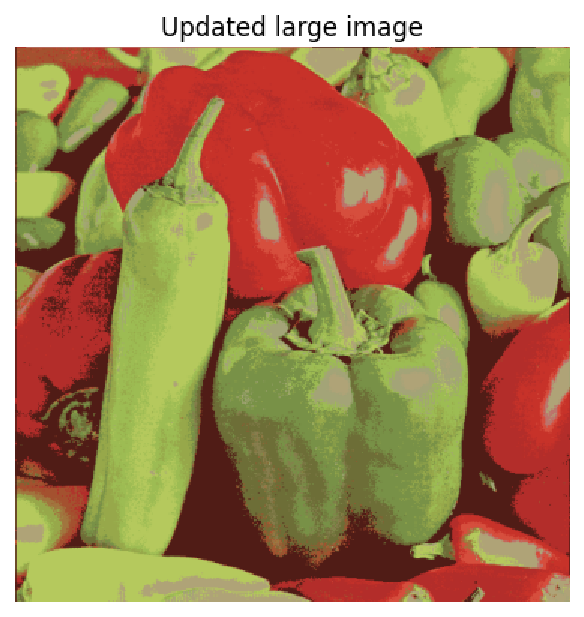
\includegraphics[width=0.5\textwidth]{updated_large.pdf}
\end{answer}

} \fi


  \item\subquestionpoints{5} \textbf{Compression Factor.}

If we represent the image with these reduced (16) colors, by
(approximately) what factor have we compressed the image?


\ifnum\solutions=1 {
  \begin{answer}
The original picture requieres 3*8=24 bits to represent one pixel. New compressed picture requires 4 bits. 24/4=6.
\end{answer}

} \fi

\end{enumerate}




\end{enumerate}

\end{document}
